% TEMPLATE for Usenix papers, specifically to meet requirements of
%  USENIX '05
% originally a template for producing IEEE-format articles using LaTeX.
%   written by Matthew Ward, CS Department, Worcester Polytechnic Institute.
% adapted by David Beazley for his excellent SWIG paper in Proceedings,
%   Tcl 96
% turned into a smartass generic template by De Clarke, with thanks to
%   both the above pioneers
% use at your own risk.  Complaints to /dev/null.
% make it two column with no page numbering, default is 10 point

% Munged by Fred Douglis <douglis@research.att.com> 10/97 to separate
% the .sty file from the LaTeX source template, so that people can
% more easily include the .sty file into an existing document.  Also
% changed to more closely follow the style guidelines as represented
% by the Word sample file. 

% Note that since 2010, USENIX does not require endnotes. If you want
% foot of page notes, don't include the endnotes package in the 
% usepackage command, below.

\documentclass[letterpaper,twocolumn,10pt]{article}
\usepackage{usenix,epsfig,endnotes}
\usepackage{alltt}  %
\usepackage{svg}
\usepackage{hyperref}
\usepackage[boxed, linesnumbered,ruled,vlined]{algorithm2e}
\usepackage[american]{babel}
\usepackage{setspace}
\usepackage{enumitem}
\usepackage{amsmath}
\usepackage{setspace}
\usepackage{float}
\usepackage{longtable}
\usepackage{booktabs}
\usepackage{caption} 
\usepackage{array}
\usepackage{graphicx}
\usepackage{subcaption}
\usepackage{tabularx}
\usepackage[table]{xcolor}
\usepackage{multirow}
\usepackage[utf8]{inputenc}
\usepackage[numbers]{natbib}
\usepackage{listings}
\usepackage{cleveref}
\usepackage{xcolor}
\usepackage{titlesec}
\usepackage{natbib}
\usepackage{tabularx} 

\begin{document}

%don't want date printed
\date{}

%make title bold and 14 pt font (Latex default is non-bold, 16 pt)
\title{\Large \bf Distributed, Linux Kernel Integrated Security Framework for
Real-Time Prevention of DNS Data Exfiltration and DNS C2}

\author{
{\rm Vedang Parasnis}\\
University of Washington, Bothell
}
% \and
% {\rm Second Name}\\
% Second Institution
% }

\maketitle

% Use the following at camera-ready time to suppress page numbers.
% Comment it out when you first submit the paper for review.
\thispagestyle{empty}


\subsection*{Abstract}
DNS-based data exfiltration remains a critical blind spot in modern infrastructure, especially for hyperscalers operating AI workloads and handling sensitive data across distributed Linux environments. In 2024, the average cost of a data breach exceeded \$4.8 million, with DNS emerging as the main exploitation channel.
This project develops the first scalable, kernel-enforced DNS exfiltration prevention framework capable of detecting and disrupting advanced Command-and-Control channels in real time. It integrates high-performance eBPF programs for deep packet inspection directly in the Linux kernel, combined with a userspace neural network for low-latency lexical analysis of advanced data obfuscation in DNS. Malicious queries trigger immediate process termination from within the kernel, cutting off exfiltration at the source before data loss or lateral movement occurs.
The framework introduces rich system level telemetry that stream process-level observability and domain-based threat intelligence to Kafka, enabling live policy enforcement and domain blacklisting across nodes without relying on external firewalls or proxies. Experimental results show detection and response speed as low as 326~$\mu$s even against stealthy, obfuscated payloads generated by industry-grade adversary emulation tools. This significantly reduces attacker dwell time and provides security teams with actionable visibility into DNS-based threats at the endpoint level, at hyperscale.

\section{Introduction}
Modern threat actors increasingly rely on covert channels and lightweight implants to persist on compromised systems and exfiltrate sensitive data before detection. These implants—often delivered via phishing or social engineering—use strong encryption, beacon intervals, and protocol tunneling to evade traditional detection techniques, bypassing firewalls and security appliances.
The Domain Name System (DNS), essential for name resolution and service discovery, is a particularly attractive channel for adversaries. Its ubiquity and general lack of deep inspection at the network edge make it an ideal vector for stealthy command-and-control (C2) and data exfiltration. Notably, campaigns by advanced persistent threats (APTs) like Hexane and MoustachedBouncer have demonstrated how encrypted DNS tunnels and ISP-level redirection can enable long-term espionage across sectors such as energy, telecom, and state institutions.
Existing DNS security approaches—anomaly detection, domain reputation scoring, and blacklist filtering—are reactive and imprecise. These methods often fail to detect adaptive or obfuscated malware behavior in real time, offering little to no assurance that damage can be prevented before data is lost or malicious commands are executed.
This work introduces a new endpoint-centric defense that enforces DNS exfiltration prevention from within the Linux kernel. Rather than relying on external monitoring systems or delayed userspace analysis, the system provides real-time, in-line protection by integrating kernel traffic control, eBPF, and userspace deep learning inference.
Our design is guided by five key goals:
\begin{itemize}[nosep]
    \item Kernel-based enforcement: Inline DNS protocol parsing within the kernel datapath through eBPF eliminates dependency on middleware and accelerates response.
    \item Instant implant disruption: Malicious DNS activity triggers immediate process termination without human intervention from within operating system.
    \item Adaptive detection: A lightweight userspace deep learning model aids in identifying obfuscated payloads missed by static heuristics.
    \item Distributed enforcement: Threat signals are streamed for scalable cross-node policy propagation and L3/L7 filtering.
    \item Broad threat coverage: Detection extends to DGAs, side channels, and remote execution beyond simple data exfiltration.
\end{itemize}

This paper details the architecture, implementation, and evaluation of our DNS exfiltration prevention security framework, showing its ability to stop DNS-based exfiltration and covert C2 in real time with low overhead massively scalable for real-world production cloud environments.


\section{Background}
\label{sec:background}

Modern threats exploit the increasing programmability of infrastructure, with adversaries leveraging stealthy implants and protocol-compliant covert channels to evade detection. Traditional kernel defenses, based on static access controls and syscall auditing, lack the dynamic enforcement needed to stop data exfiltration in real time. Technologies like P4 or DPDK offer programmable data planes but operate outside core kernel security paths. They rely on user-space poll-mode drivers or offload via NIC firmware, making them unsuitable for enforcing endpoint security across kernel subsystems like LSMs, syscalls, or tracepoints.

The extended Berkeley Packet Filter (eBPF), introduced in Linux 3.15, enables safe and efficient programmability inside the kernel. eBPF programs are written in a restricted C dialect, verified by the kernel for memory and control safety, JIT-compiled, and attached to various hooks including networking, system calls, and LSMs. Persistent state is maintained using in-kernel BPF maps, supporting complex structures like LRU caches or per-CPU arrays. This makes eBPF uniquely capable of enforcing context-aware, low-latency security policies directly at the point of execution.

Within the networking stack, eBPF integrates deeply via Traffic Control (TC), particularly through the \texttt{clsact} qdisc, which enables deterministic filtering on both ingress and egress paths. This allows enforcement without interfering with existing QoS mechanisms or requiring changes to traffic class hierarchies. While TC is heavily used in Kubernetes for overlay networking and node communication, its security enforcement potential is underutilized—particularly at the endpoint where lateral movement or exfiltration often begins.

DNS is a prime target for covert channels due to its ubiquity, loose filtering, and limited visibility. Implants encode sensitive data into the subdomain portion of DNS queries using base encodings, XOR masks, encryption, or segmentation, and transmit them to attacker-controlled domains via recursive resolution. Table~\ref{dns_payload_obfuscation} summarizes representative obfuscation strategies. DNS tunneling extends this by embedding entire payloads within DNS queries, while DNS-based C2 allows bi-directional control via encoded responses. Even noisier strategies like raw DNS exfiltration can succeed before thresholds trigger alerts.

\begin{table}[htbp]
\footnotesize  % Reduce font size for better fit
\centering
\caption{DNS Payload Obfuscation Examples}
\begin{tabularx}{\linewidth}{@{}llX@{}}
\toprule
\textbf{Technique} & \textbf{Payload} & \textbf{Encoded Subdomain} \\
\midrule
Base64     & TopSecret & VG9wU2VjcmV0.dns.exfil.com \\
XOR (0xAA) & TopSecret & DE.D5.F2.F9.E9.C7.CF.DE.dns.exfil.com \\
NetBIOS    & TopSecret & ECPFEDFEFCDCECEEEA.dns.exfil.com \\
CRC32      & TopSecret & 7F9C2BA4.dns.exfil.com \\
AES-CBC    & TopSecret & IV.A1.B2.C3.D4.E5.F6.07.08.dns.exfil.com \\
RC4        & TopSecret & 9A.B3.47.E2.8C.4D.11.6F.dns.exfil.com \\
Raw Hex    & TopSecret & 546f70536563726574.dns.exfil.com \\
\bottomrule
\end{tabularx}
\label{dns_payload_obfuscation}
\end{table}


Standardized DNS enhancements such as DNSSEC and DNS-over-TLS (DoT) aim to improve integrity and privacy. However, DNSSEC does not encrypt queries, and DoT hinders deep packet inspection and blind intrusion detection systems (IDS). These measures fail against endpoint-resident implants that use legitimate-looking DNS traffic for covert operations.

Existing defenses—such as DNS sinkholing or Response Policy Zones (RPZ)—are effective only against known threats. They rely on static blacklists or post-facto deep packet inspection, making them reactive. Against adaptive implants using DGA, ephemeral keys, or randomized timing, these mechanisms are too slow to prevent real-time data theft or command execution. A more proactive, kernel-level enforcement mechanism is needed to terminate the threat path at its source—before damage occurs.

\section{Related Work}
\label{sec:related-word}
This section reviews prior work in three areas: eBPF-based network security, machine learning for DNS exfiltration detection, and enterprise-grade DNS defenses.


\subsection{Network Security Using eBPF}
eBPF has become foundational in Linux-based networking, security, and observability. It allows safe, verifiable code to run in the kernel, supporting high-throughput enforcement without kernel modification. XDP (eXpress Data Path) is commonly used for high-speed packet drops at the NIC level and is effective for DoS/DDoS mitigation~\cite{10.1145/3281411.3281443, 8850758}. Studies have examined eBPF's architectural characteristics and performance~\cite{10.1145/3371038, bertrone2018accelerating}, though most focus on ingress traffic.

A recent study explored eBPF with XDP to mitigate DNS water torture DDoS attacks on authoritative servers~\cite{9165454}, and another proposed XDP-based TCP SYN and UDP flood mitigation~\cite{bertin2017xdp}. However, both techniques overlook low-throughput, stealthy DNS exfiltration.

DNSXP~\cite{8725640, steadman2021dnsxp} remains one of the few eBPF-based systems for DNS exfiltration defense. It combines SDN with eBPF at the XDP layer, enabling early filtering but only on ingress. Reliance on static rules limits adaptability, and packet mirroring to an SDN controller introduces latency, allowing exfiltration before detection.

Cilium supports eBPF-based network policies at layers 3–7~\cite{zavarella2022methodology, 10.1145/3651890.3672227}, enabling L7-aware DNS filtering. However, it lacks dynamic blacklisting and egress-focused inspection. Microsoft’s Inspector Gadget and other tools also rely on userspace rules and do not offer deep kernel-level enforcement. These limitations highlight the need for a dynamic, distributed, egress-aware kernel security system for DNS traffic.

\subsection{Machine Learning for DNS Exfiltration Detection}
Machine learning approaches have significantly advanced DNS anomaly detection. Many systems use traffic volume, rate, and lexical features to identify potential exfiltration or C2 patterns~\cite{apt-process, Das, 8717806d}. However, most operate post-factum, focusing on detection over prevention.

Passive DNS analysis platforms such as EXPOSURE and NOTOS~\cite{bilge2011exposure, antonakakis2010building} extract features from large datasets to detect botnets and C2 domains but lack enforcement capability. Other efforts use entropy, timing, or lexical models to detect low-throughput DNS tunneling~\cite{DBLP:journals/corr/abs-1709-08395, 10.1145/3230833.3233278}, but these models are reactive and can miss slow or evasive tactics.

Mobile agent-based mitigations introduce latency and suffer from false positives~\cite{9486400}. The C2 Eye framework~\cite{haider2024c2} detects attacks in software supply chains but lacks protection against the damage they cause in real time. Process DNS~\cite{sivakorn2019countering} correlates DNS traffic with userspace processes but remains vulnerable to kernel bypasses, privilege escalation, and lacks enforcement via kernel mechanisms.

These solutions are limited by userspace-only architectures and lack in-kernel context, port-layer obfuscation visibility, or fine-grained security policy enforcement. They are passive, often offline, and ineffective against modern tactics such as remote shell access, dynamic DGAs, or multiplayer C2s. No current system enforces real-time DNS payload prevention with egress-side blocking, process termination, dynamic domain updates, and cloud-native deployment capabilities.

\subsection{Enterprise DNS Security Solutions}
Enterprise firewalls like Akamai and AWS Route 53 employ anomaly-based detection and domain-based filtering. Akamai’s ibHH algorithm tracks information-heavy subdomain transmissions~\cite{ozery2023information}, while AWS detects tunneling and DGAs using volume thresholds~\cite{ansari2020reinforcing}. However, these systems operate at the DNS server level and lack direct endpoint enforcement.

Route 53 lacks cross-protocol observability, and AWS Network Firewall does not enforce L3-layer payload-level filtering on DNS traffic. Cloudflare and Broadcom's Carbon Black offer partial DNS defenses but focus primarily on DDoS or rely on userspace-based behavior models~\cite{ahmed2019monitoring}.

Infoblox extends DNS filtering using threat intelligence, and Carbon Black includes process blocking. Yet both rely on userspace agents and cannot correlate low-level system behavior or prevent payload leakage from within the kernel. None of these systems support in-kernel DNS payload inspection, dynamic blacklist enforcement, or kernel-integrated mitigation.


\subsection{Related work summary}
Across academic and enterprise domains, no solution provides low-latency, egress-side, kernel-enforced DNS security. Userspace-only architectures are slow, prone to evasion, and blind to NIC-layer traffic. Kernel-aware defenses—capable of terminating malicious implants and dynamically enforcing policy—are necessary to protect against covert DNS-based data exfiltration in real time.



\section{Proposed Approach}



\section{Implementation and Evaluation}
This section evaluates the effectiveness of the implemented DNS exfiltration prevention security framework in a distributed setting with comprehensive evaluation results and analysis.




\subsection{Environment Setup}
The security framework developed was deployed on eight CSSVLAB nodes (CSSVLAB{01–08}), each running Ubuntu 24.02 with Linux kernel 6.12 on Intel Xeon Gold 6130. Each node had 8GB RAM and 24GB storage. The systems ran under the \texttt{netvsc} hypervisor network driver, with 100 Gbits/sec network bandwidth and 8 TX/RX hardware queues aligned to CPU cores to enable optimal packet steering and parallel processing for high-throughput netflow handling. In addition, all eight CPU cores and memory resided on a single NUMA node, eliminating memory lookup overhead during kernel benchmarking. The test bench launches a custom PowerDNS authoritative and recursor server on CSSVLAB08. The controller and a Kafka single broker instance run on CSSVLAB01. Nodes CSSVLAB{02–07}, excluding CSSVLAB06, act as the data plane, each running the eBPF agent and using the custom PowerDNS server as the default resolver via systemd-resolved. CSSVLAB06 is used to simulate DNS exfiltration attacks against data plane nodes, tunneling DNS queries through the same PowerDNS instance. The complete deployment is illustrated in Figure~\ref{fig:deployed-arch}


\subsection{Evaluations Results}
The evaluation of this security framework is presented for each individual architecture sub-component in the following sections.


\subsection{Data Plane}
The effectiveness of the eBPF agent at the endpoint of the data plane is evaluated through quantized deep learning model metrics, comparison of DNS request throughput in both operational phases (active and passive), and measurement of bandwidth and resource utilization, including CPU and memory usage, as well as throughput of kernel events processing. Finally, the agent’s resilience coverage against advanced adversary emulation frameworks including agent's response time for these attacks is evaluated. Agent's performance evaluation is performed on a single node within the data plane running the eBPF agent at the endpoint.


\subsubsection{Deep Learning Model Evaluation}
The trained deep learning model was evaluated on a dataset of 3.8 million domains, divided into 70\% for training and 15\% each for validation and testing. After training, the model achieved a validation precision of 99.7\%, with the loss steadily decreasing throughout the 25 training epochs and reaching 0.98\% at the end, as shown in Figure~\ref{fig:model_precision}. Given the DNS data exfiltration use case, the model performance was assessed with a primary emphasis on minimizing false positives. A high false-positive rate would not only cause the eBPF agent to drop benign DNS packets and generate false threat events, but could also result in the termination of legitimate processes, thereby introducing operational risks. In contrast, false negatives were considered less critical, as the agent would allow malicious traffic to pass through without taking privilege-level actions. Therefore, \textbf{precision} was prioritized over recall. These metrics are formally defined as:
\[
\text{Precision} = \frac{\text{TP}}{\text{TP} + \text{FP}},
\]
% while recall is defined as:
\[
\text{Recall} = \frac{\text{TP}}{\text{TP} + \text{FN}}.
\]
Based on these considerations, and using a data set engineered to capture a wide range of data obfuscation techniques, the model achieved a precision of 99.59\% and a recall of 99.87\% when evaluated on the test dataset, as shown in Figure~\ref{tab:model-evaluation-metrics}, with the corresponding confusion matrix presented in Figure~\ref{fig:conf-matrix}.
For runtime inference using ONNX within the eBPF agent, a binary classification threshold of 0.85 was selected. This value was determined by analyzing F1 score performance across varying classification thresholds, as illustrated in Figure~\ref{fig:model_f1_threshold}, with particular attention to the trade-off between precision and recall. Since minimizing false positives was the top priority, the selected threshold maximized precision while maintaining a relatively high recall.
This high-precision, low false-positive outcome was enabled by the chosen feature set, which included Shannon entropy across multiple encoding and encryption schemes, allowing the model to effectively learn obfuscation patterns.

\begin{figure}[t]
  \centering
  \subfloat[Model Evaluation Metrics]{%
    \begin{minipage}[t]{0.45\linewidth}
      \centering
      \small
      \begin{tabular}{@{}lcc@{}}
        \toprule
        \textbf{Metric} & \textbf{Train} & \textbf{Test} \\
        \midrule
        Accuracy & 0.9973 & 0.9997 \\
        AUC & 0.9997 & 0.9997 \\
        Loss & 0.0099 & 0.0091 \\
        Precision & 0.9959 & 0.9959 \\
        Recall & 0.9987 & 0.9988 \\
        \bottomrule
      \end{tabular}
    \end{minipage}
  }
  \hfill
  \subfloat[Confusion Matrix]{%
    \begin{minipage}[t]{0.48\linewidth}
      \centering
      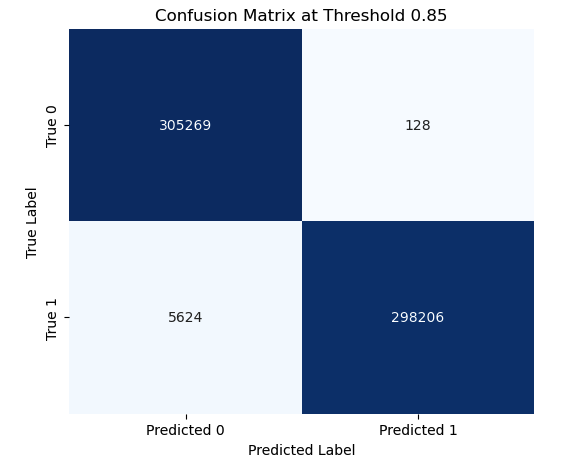
\includegraphics[width=\linewidth]{images/results/model/confusion_matrix.png}
    \end{minipage}
  }
  \caption{Model performance summary including evaluation metrics and confusion matrix.}
  \label{fig:model-summary}
\end{figure}


\begin{figure*}[t]
  \centering
  \subfloat[Model Precision]{%
    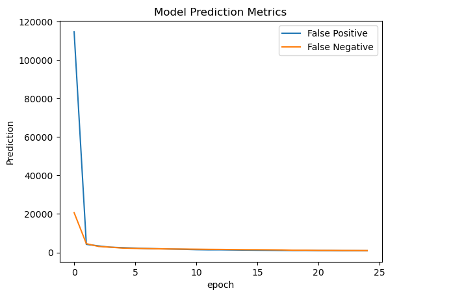
\includegraphics[width=0.48\textwidth]{images/results/model/mpred.png}
    \label{fig:model_precision}
  }
  \hfill
  \subfloat[Precision, Recall, and F1 Score vs. Threshold]{%
    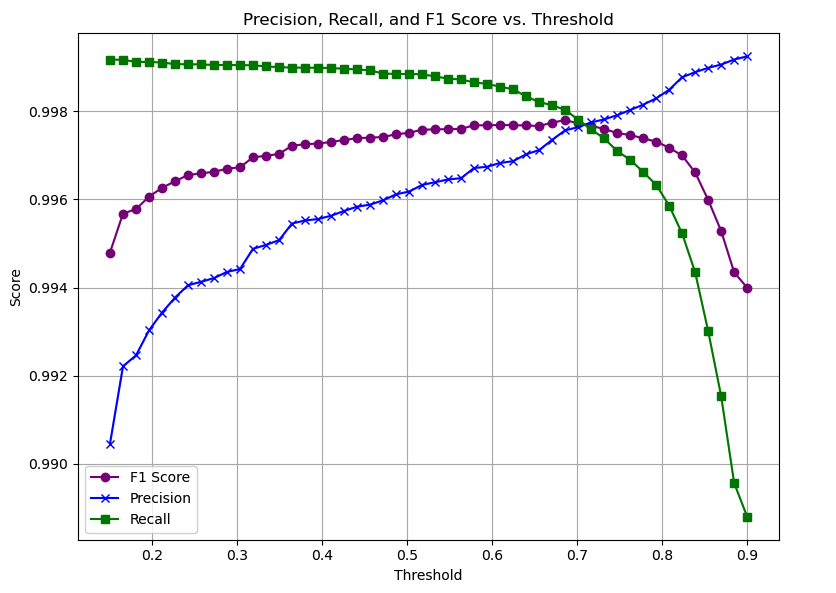
\includegraphics[width=0.48\textwidth]{images/results/model/f1_score.png}
    \label{fig:model_f1_threshold}
  }
  \caption{Precision and F1 score analysis of the deep learning model under varying decision thresholds.}
  \label{fig:threshold-performance}
\end{figure*}


\subsubsection{Effectiveness of eBPF Agent Against DNS Exfiltration Frameworks}
The eBPF agent was evaluated across all data plane endpoints against widely used DNS-based C2 frameworks commonly employed by red teams. Tests focused on disrupting C2 and exfiltration activity tunneled through DNS, with CSSVLAB06 serving as the attacker node. The BishopFox Sliver framework was tested in agent's active mode for both basic exfiltration and advanced operations, including remote shell access, code execution, file transfers, port forwarding, and persistence, entirely over DNS. The agent intercepted the initial C2 packet at the kernel level, immediately disrupting communication, triggering retries, and terminating implants for both beacon-based and session-based channels. Since Sliver lacks randomized UDP port support, transport obfuscation was assessed using dnscat2. In both active and passive modes, the agent enforced mitigation policies, leading to full-session termination and zero data exfiltration. The average response time for each measured exfiltration attempt was 316.233 microseconds, as shown in Figure~\ref{fig:response_speed}. For raw exfiltration, tools such as DET were immediately blocked. Furthermore, iodine, which tunnels through TUN/TAP interfaces, was effectively mitigated. All other bulk exfiltration tools were similarly thwarted. Table~\ref{tab:dns-framework-coverage} summarizes the tools tested and the associated attack vectors prevented.

\begin{figure}[t]
  \centering
  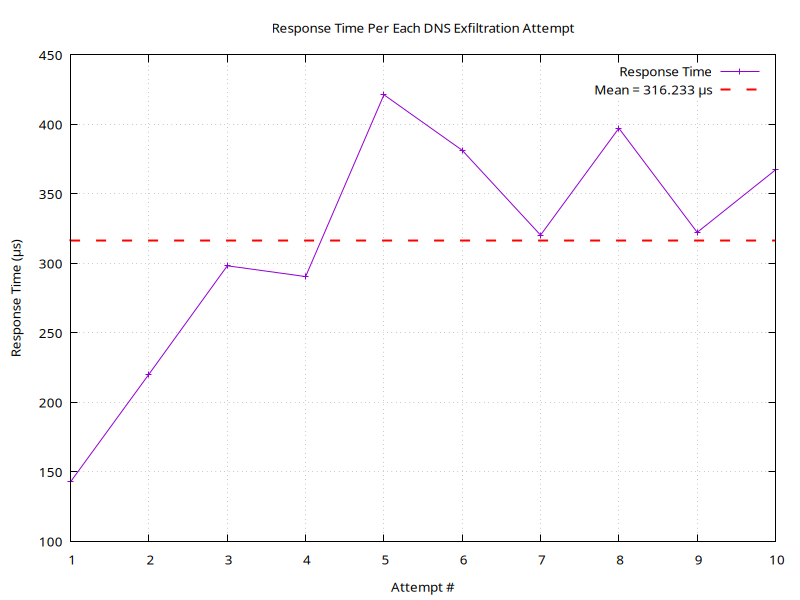
\includegraphics[width=\linewidth]{images/results/response_speed/response_speed.png}
  \caption{eBPF Agent: Response Time for Each DNS Exfiltration Attempt}
  \label{fig:response_speed}
\end{figure}



\begin{figure}[t]
  \centering
  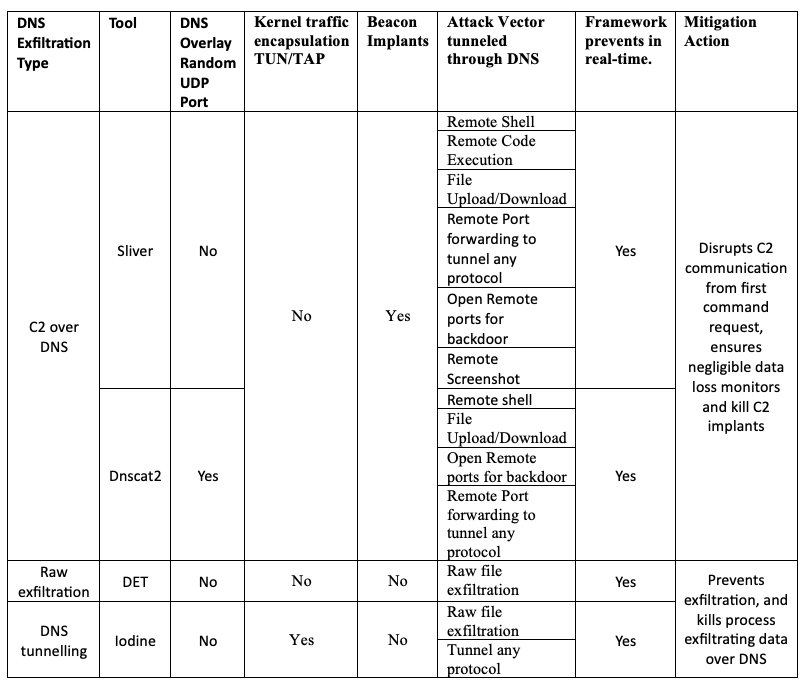
\includegraphics[width=0.85\linewidth]{images/results/C2_exfil_strength.png}
  \caption{Framework Coverage Against Real-World DNS C2 and Exfiltration Tools}
  \label{tab:dns-framework-coverage}
\end{figure}

% \begin{figure}[h]
% \centering
% 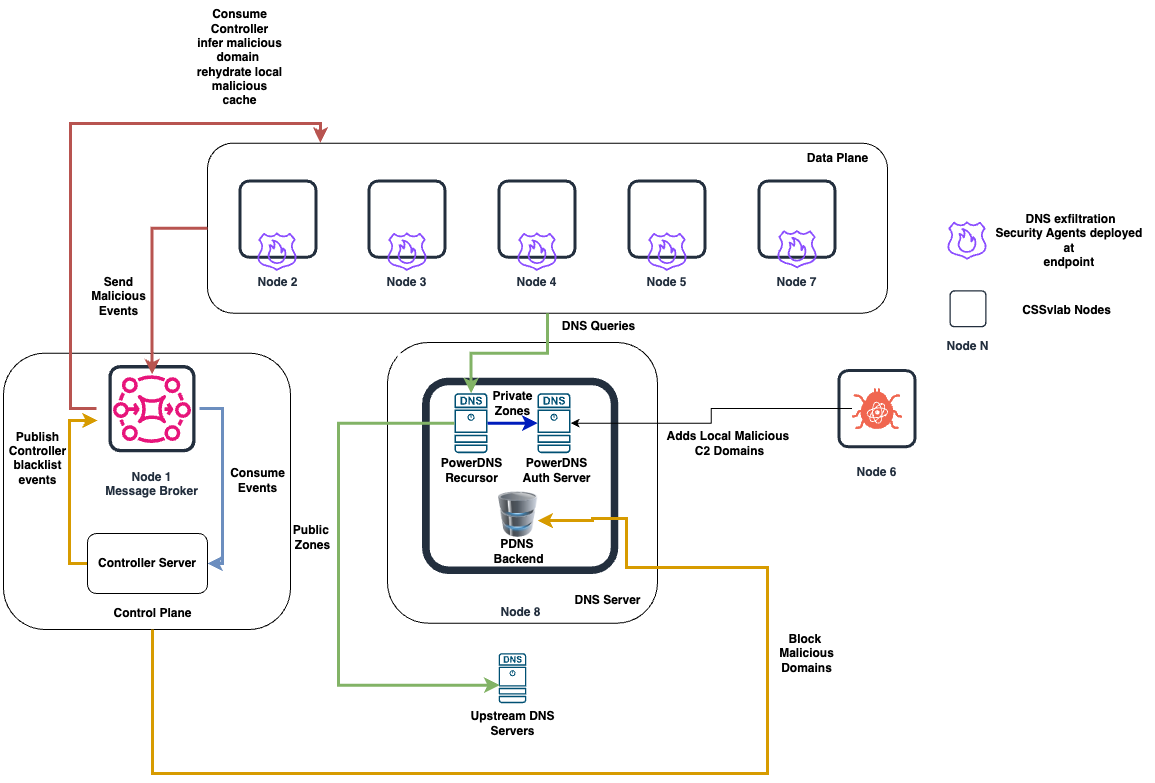
\includegraphics[width=1.0\textwidth]{UWThesis/images/cssvlab-arch.png}
% \caption{Security Framework Deployed Architecture over CSSVLAB Nodes}
% \label{fig:deployed-arch}
% \end{figure}




\section{Conclusion}
\label{sec:conclusion}

\subsection{Summary}
This framework advances the state of the art in DNS exfiltration prevention by introducing a kernel-enforced, horizontally scalable security architecture designed for modern cloud deployments. Existing solutions—centered on centralized detection, userspace anomaly systems, or proxy-based deep packet inspection—fail to detect or stop sophisticated DNS-based command-and-control (C2) attacks. In contrast, this work introduces a new security layer: real-time endpoint protection from within the kernel itself.

By reprogramming kernel subsystems via eBPF and incorporating deep learning–based inference, the framework enforces system-wide DNS security and offers process-level mitigation. It blocks covert DNS channels, terminates implants, and detects advanced threat vectors modeled by top-tier adversary emulation platforms.

The architecture combines kernel-level enforcement with endpoint-centric observability, enabling rich metrics and fast response while maintaining low-latency scalability. The following summarizes its key capabilities:

\begin{itemize}[nosep]
    \item \textbf{Real-Time DNS C2 Disruption} – Immediately blocks DNS-based command-and-control traffic at the kernel level.
    
    \item \textbf{Process-Level Detection and Termination} – Actively monitors and terminates processes using DNS for covert exfiltration.
    
    \item \textbf{Encapsulation-Aware Defense} – Detects and blocks DNS tunneling and DNS-over-random-port techniques within the kernel, independent of transport protocol.
    
    \item \textbf{Mitigation of Advanced DNS C2 Techniques} – Stops attacks involving reverse shells, file transfer, protocol tunneling, remote port forwarding, and multi-stage or multiplayer C2 channels.
    
    \item \textbf{Dynamic DGA Detection and Network Policy Enforcement} – Blacklists domains in real time and reprograms network policy agents for cross-protocol enforcement at Layer 3.
    
    \item \textbf{System Observability and Metrics} – Integrates with Prometheus to provide fine-grained observability and telemetry across distributed data plane nodes.
\end{itemize}

\subsection{Limitations}
While the framework demonstrates strong performance in real-time prevention, several limitations remain:

\begin{itemize}[nosep]
    \item \textbf{Latency in Active Mode} – Redirecting DNS-over-UDP traffic from the kernel to userspace for inference introduces latency. However, this remains lower than proxy-based DPI. In latency-sensitive deployments, enforcement aggressiveness can be tuned at runtime.
    
    \item \textbf{Fork-Based Evasion in Passive Mode} – In passive mode, attackers may evade detection by forking child processes. This can be mitigated by tracking malicious ancestry via the kernel \texttt{task\_struct} instead of relying solely on PID-based correlation.
    
    \item \textbf{Inference Bottlenecks} – The Python-based ONNX server introduces concurrency and throughput limitations due to Python’s GIL and IPC overhead. Future migration to a compiled, concurrent runtime is required.
    
    \item \textbf{Lack of Encrypted DNS Support} – The framework currently does not prevent DNS exfiltration over encrypted channels such as DoT or DoH.
    
    \item \textbf{No Coverage for Encrypted Tunnels} – Traffic within kernel-encrypted tunnels (e.g., WireGuard, OpenVPN, IPSec) bypasses DNS-layer enforcement. Integration with \texttt{xfrm} hooks is required.
\end{itemize}

\subsection{Future Work}
Several extensions can further enhance the framework’s capability:

\begin{itemize}[itemsep=1pt,parsep=0pt]
    \item \textbf{Support for DNS-over-TCP and TLS Tunnels} – Extend eBPF programs to track stateful DNS over TCP traffic and integrate an L7 proxy (e.g., Envoy) to handle encrypted payloads.
    
    \item \textbf{High-Performance Inference via Rust or WebAssembly} – Replace the Python ONNX inference pipeline with a Rust or Wasm-based runtime to improve throughput and concurrency on multi-core systems.
    
    \item \textbf{Kernel-Level TLS Fingerprinting} – Implement JA3/JA4 fingerprinting using eBPF to detect encrypted C2 exfiltration over TLS, supporting behavior-based classification in userspace.
    
    \item \textbf{Volume-Based DNS Rate Limiting} – Add DNS egress throttling via HTB and \texttt{EDT\_BPF} to block large-volume exfiltration attempts at line rate.
\end{itemize}


% Some embedded literal typset code might 
% look like the following :

% {\tt \small
% \begin{verbatim}
% #include <iostream>
% using namespace std;
% main()
% {
% cout << "Hello world \n";
% return 0;
% }

% \end{verbatim}
% }

% Now we're going to cite somebody.  Watch for the cite tag.
% Here it comes~\cite{Einstein}.  

% Lorem ipsum dolor sit amet, consectetur adipiscing elit, sed do eiusmod tempor incididunt ut labore et dolore magna aliqua. Ut enim ad minim veniam, quis nostrud exercitation ullamco laboris nisi ut aliquip ex ea commodo consequat. Duis aute irure dolor in reprehenderit in voluptate velit esse cillum dolore eu fugiat nulla pariatur. Excepteur sint occaecat cupidatat non proident, sunt in culpa qui officia deserunt mollit anim id est laborum.

% Lorem ipsum dolor sit amet, consectetur adipiscing elit, sed do eiusmod tempor incididunt ut labore et dolore magna aliqua. Ut enim ad minim veniam, quis nostrud exercitation ullamco laboris nisi ut aliquip ex ea commodo consequat. Duis aute irure dolor in reprehenderit in voluptate velit esse cillum dolore eu fugiat nulla pariatur. Excepteur sint occaecat cupidatat non proident, sunt in culpa qui officia deserunt mollit anim id est laborum.

% Lorem ipsum dolor sit amet, consectetur adipiscing elit, sed do eiusmod tempor incididunt ut labore et dolore magna aliqua. Ut enim ad minim veniam, quis nostrud exercitation ullamco laboris nisi ut aliquip ex ea commodo consequat. Duis aute irure dolor in reprehenderit in voluptate velit esse cillum dolore eu fugiat nulla pariatur. Excepteur sint occaecat cupidatat non proident, sunt in culpa qui officia deserunt mollit anim id est laborum.

% Lorem ipsum dolor sit amet, consectetur adipiscing elit, sed do eiusmod tempor incididunt ut labore et dolore magna aliqua. Ut enim ad minim veniam, quis nostrud exercitation ullamco laboris nisi ut aliquip ex ea commodo consequat. Duis aute irure dolor in reprehenderit in voluptate velit esse cillum dolore eu fugiat nulla pariatur. Excepteur sint occaecat cupidatat non proident, sunt in culpa qui officia deserunt mollit anim id est laborum.

{\footnotesize \bibliographystyle{acm}
\bibliography{sample}}


% \theendnotes

\end{document}







